\section{Overall Task Description}
We can consider each of the queries to be a logistic regression problem from image space to a binary answer (as all questions we currently train on are yes or no questions), and thus the meta-learning aspect comes in examining how much previously acquired queries help reduce the amount of training required to learn subsequent queries. The closest parallel in the literature is the visual question answering (VQA; \cite{Antol2015}) paradigm. Our task offers a different focus than those two existing ones: VQA primarily investigates integrating natural language understanding with visual reasoning, and CLEVR offers more uniform images and a smaller range of queries but challenges relational reasoning between objects. Our task modifies the stimuli, simplifying some aspects (visual noise, number of objects) and complicating others (number of colors, shapes, and materials) and removes the language component to allow focusing on meta-learning algorithms’ scaling performance. As currently formulated, this task also differs from other supervised computer vision problems: image classification requires assigning a single label to an object, and multilabel classification does not usually involve an explicit query. Semantic segmentation (labeling each pixel as part of an object) is a much harder visual task, with a substantially different output (a pixel map segmenting the image), and image captioning requires reasoning over similar visual information, but again, excluding a query and expecting a different form of output (a textual description).

Note that this task structure by itself does not necessarily investigate meta-learning. However, the structure of the task and dataset are crucial to the design of the two benchmark paradigms we propose, which do allow evaluating meta-learning capabilities:

\section{The Sequential Benchmark}
In this benchmark, we examine if and how much a model learns how to generalize between queries in the same dimension. Does learning to answer a few color-related questions help learn the next color related task more efficiently? To test this, we sequentially expose the model to tasks in a single dimension. In the first episode, we begin with a single task (\textit{`Is there a red object?'}), and train the model on it until it reaches criterion (95\% accuracy on the held-out test set). In the second episode, we add a second task to the training set (\textit{`is there a blue object?'}), retaining the first task in the training set (rather than continuing training only on the new one), in order to avoid catastrophic forgetting, and resume training and testing until reaching criterion on the test set in both tasks. If we do not set the criterion to be on both tasks, the model quickly forgets earlier tasks, as Figure \ref{fig:old-sequential-benchmark} demonstrates. We continue to mix in a new task in every episode in such a fashion, examining the time required to train each additional task to reach the threshold criterion. We wish to examine the amount of training (in total iterations performed) required to achieve criterion in each additional task, which would ideally asymptote toward some minimum, varying by the model architecture examined. We currently transition to the next task based on the held-out test set accuracy, but we realized in retrospect that it would be sensible to introduce a validation set for that purpose. Theoretically, by transitioning based on the test set, we allow it to influence the progress on the benchmark, and it would be preferable to do that based on a validation set and maintain an independent test set. However, since we do not allow the model to learn on these examples, and do not use them for hyperparameter selection, this should not raise an issue, since the same generative process would create the validation and test sets. We will consider introducing it should we revisit this benchmark in the future.  
\begin{figure}[!htb]
% \vspace{-0.225in}
\centering
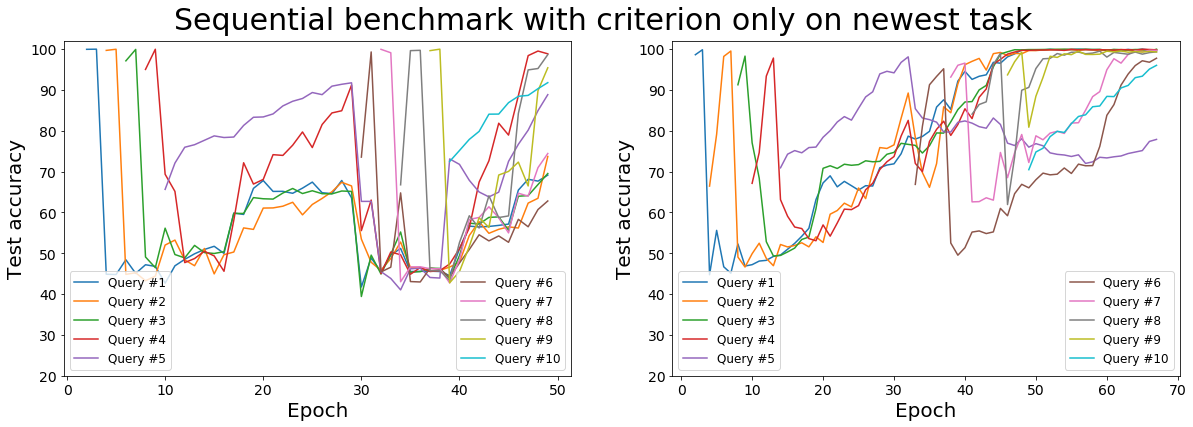
\includegraphics[width=\linewidth]{ch-dataset-task-benchmark/figures/benchmark/old_benchmark.png}
\caption[Sequential benchmark with criterion only on newest task.]{{\bf Sequential benchmark with criterion only on newest task.} The results of two example sequential benchmark iterations (using slightly different coreset settings and different random seeds) with the accuracy criterion only on the newest task. While in the right-hand side plot most query accuracies eventually improve, in the left-hand side plot many tasks fail to reach criterion. These results motivated setting the accuracy criterion to all tasks, rather than only the more recent task.}
\label{fig:old-sequential-benchmark}
% \vspace{-0.2in}
\end{figure}

To focus on the current task while maintaining previous tasks, we modify the coreset approach described by \textcite{Nguyen2018}. In every epoch, we assign a single query to each of the 45,000 training set images. We assign one half of the training set (22,500 images) to the current task learned, and the remaining 22,500, the coreset, are split as evenly as possible between the previously trained queries. On every epoch, we sample a new appropriately sized coreset for each previous task. We require the coreset not to be extremely imbalanced: if the ratio of positive to negative examples (in either way) is more than 4:1, or in other words, if either positive or negative examples reflect under 20\% of the coreset for a given task, we sample it again. After sampling the coreset, we assign the remaining 22,500 images to the current task and begin training. 

Note that as we acquire additional previous tasks, each one receives fewer coreset examples in every epoch. The diminishing repetition of past tasks could also be viewed as a sort of distributed practice, which relies on the spacing effect, as a method of improving memory recall (cf. \cite{Bahrick1993}; \cite{Russo1998}). We treat the test set in a more standard fashion, evaluating each of the 5000 test set images using all active (current and previous) queries.

To avoid sensitivity to the order in which we introduce the tasks, we average this scaling behavior over several different executions, each execution adding the tasks in a different order. To further mitigate the potential for order-related effects, we employ a Latin square design (see \cite[][ch. 9]{Bailey2008}), which guarantees that for each ten-replication block, each task will appear in each ordinal position (first, second, and so on) exactly once. We do not currently account for second-order effects (how often a task appears before or after another task). To generate these designs, we take a standardized Latin square (which has the first row and column both perfectly ordered), permute the rows once and columns once, and take the appropriate row for the index within the current ten-replication block \parencite{InteractiveStatisticalPages}. When comparing different models, we will use the same random seed for the row and column permutation, guaranteed we compare on identical column orderings. 

We currently investigate each dimension independently, examining different orderings of the colors, shapes, and materials. There is a stronger shared structure when training only within a single dimension, which should make the meta-learning problem easier. We also developed a control condition, which attempts to examine how the degree of shared structure between the tasks helps accelerate training. Rather than train on all ten tasks from a single dimension, we train on random sets of ten tasks across all three dimensions. To control for the order of introduction between the dimensions, we cycle through the six permutations of dimension orderings\footnote{Color-shape-texture, color-texture-shape, shape-color-texture, shape-texture-color, texture-color-shape, texture-shape-color.}, sampling a task from each dimension until we reach a set of ten. We then train on these ten tasks following the benchmark protocol outlined in this section. If the model learns to exploit shared structure within a dimension, it might be slower in this condition than in the single-dimension condition, since the model has a lower degree of shared structure to exploit between the tasks. However, if the model shows benefits from overall improved visual processing, this condition might not be more difficult, and in fact, might elicit lower interference between the tasks learned.

This task allows us to explicitly evaluate how learning scales as a function of the number of previously learned related tasks. We can measure how many training examples does it take to learn a task for the first time, as a function of how many tasks have been previously learned. We can also measure how many examples it takes to re-learn a task, to overcome the interference introduced by adding a new task, as a function of the number of times the task has already been relearned. We can also quantify the catastrophic interference induced by adding additional tasks, both as a factor of how many tasks the model already knows and as a factor of how many times the model was trained on a particular task. The benchmark we describe is not unlike the incremental learning setting suggested by \textcite{Kemker2017a}, although our coreset of previous task examples aids models in retaining previous tasks, which the authors there do not afford, making their setting more challenging.

A note regarding terminology: we borrow the term \emph{episode} from the meta-learning literature, and use it to refer to each stage in the benchmark with a fixed number of tasks. In other words, the benchmark is comprised of ten episodes, the first with one task, and the second two, and the last with ten. Each episode requires one or more \emph{epochs} to complete, where an epoch is one pass through the entire training set, with each training example allocated to a single active task. 

\section{The Compositional Benchmark}
The description of this benchmark will be less detailed than the previous one since this is a second benchmark we foresee implementing with this dataset and task structure but have not implemented yet. We describe it to demonstrate additional investigations this dataset and task structure would allow us to pursue: 

In this benchmark, we will examine a different sort of meta-learning: if a model learns two parts of a composite query, does it make it easy (or ideally, immediate) to learn composite queries as well? We can consider several different phases of this benchmark: in the first, we train a model on several single-item tasks (``Is there a red object?'' ``Is there a torus'') until reaching criterion. Once the model performs adequately on these tasks, we begin training on composite tasks (``Is there a red torus?''), composed entirely from tasks the model reached criterion on, monitoring how much additional training is required to achieve criterion on these conjunctive tasks from previously-trained single-item queries. 

In the second phase, we introduce additional features in each dimension without training on them individually. We now train on composite queries involving one previously trained feature and one new one (\textit{`Is there a red pyramid?’ `Is there a teal torus?’}), again training until reaching an accuracy threshold on all such queries. In the final training phase, we introduce the remaining colors, materials, and textures, and examine how much additional training is required for learning their conjunctive queries. As in the previous phase, we do not train on the single-item queries. The training is complete once the model reaches the accuracy criterion on all two-item conditions. 

To evaluate the quality of representations learned, and go beyond the number of iterations required to finish the benchmark, we can evaluate the models on all single-item queries. As this benchmark is currently formulated, we train the models on the single-item queries only on the features introduced in the first phase. If a model learns to exploit the shared structure between items, it should fare well on the individual queries as well. Performing this additional test would allow us to not only quantify the scaling behavior as a function of compositionality but additionally the robustness and quality of representations learned. 

As with the previous benchmark, we would randomize the order in which tasks are introduced to the model, employing a similar Latin square design to the previous benchmark. The task order implies which features/tasks are trained on individually, and which ones are only introduced as part of the composite tasks. We would average over different such random training subsets to evaluate each model, but make sure to evaluate all models on the same task orderings, to make sure the comparison is valid. 
